\chapter{Agentes}

\section{Agentes inteligentes}

\begin{displayquote}
\textit{Un agente inteligente es un sistema de ordenador, situado en algún entorno, que es capaz de realizar acciones de forma autónoma y que es flexible para lograr los objetivos planeados.}
\end{displayquote}

El agente recibe entradas sensoriales del entorno donde está situado y realiza acciones que lo cambiar, actuando sin la intervención directa de humanos y con control sobre sus propias acciones y estado interno.
Estas acciones presentan un componente de flexibilidad en tanto a que pueden proceder de tres maneras diferentes:

\begin{itemize}
	\item\textbf{Reactiva:} Percibe el entorno y responde temporalmente a los cambios ocurridos en el mismo.
	\item\textbf{Pro-activa:} No actúan únicamente en respuesta a su entorno, sino que son capaces de mosrar comportamientos dirigidos a conseguir objetivos oportunos tomando la iniciativa en el momento apropiado.
	\item\textbf{Social:} Son capaces de interactuar, cuando sea apropiado, con otros agentes artificiales o humanos para completar su propio proceso de resolución del problema y ayudar a otros con sus actividades.
\end{itemize}

\subsection{Sistemas basados en agentes}

Un sistema basado en agentes (SBA) es un sistema en el que la abstracción clave utilizada es la del agente.
Un sistema multi-agente (SMA) es un SBA diseñado con varios agentes que interactúan entre sí, de forma que pueden representar problemas con múltiples métodos y entidades de resolución y perspectivas.

Los agentes interactúan entre sí de tres formas fundamentales:

\begin{itemize}
	\item\textbf{Cooperación:} Los agentes trabajan juntos para resolver un problema.
	\item\textbf{Coordinación:} Los agentes organizan una actividad para evitar las interacciones perjudiciales y explotar las beneficiosas.
	\item\textbf{Negociación:} Los egentes llegan a un acuerdo que sea aceptable por todas las partes implicadas.
\end{itemize}

Los SMA forman una IA distribuida mediante una red de resolutores de problemas que trabajan conjuntamente para resolver problemas que están más allá de las capacidades o del conocimiento de cada agente individual.
En ellos, cada agente tiene información incompleta sobre el problema o una porción de las capacidades necesarias para su resolución, gozando cada uno de un punto de vista limitado.
Se caracterizan por la inexistencia de un sistema de control global en el que los datos no están centralizados y la computación es asíncrona.

Las técnicas de cooperación son una herramienta fundamental en la formación de equipos de agentes, como es el caso de la RoboCup, mientras que las técnicas de negociación son una técnica para la coordinación y resolución de conflictos.

\section{Arquitecturas de agentes}

\subsection{Arquitecturas deliberativas}

Las arquitecturas deliberativas se basan en un \textbf{sistema de símbolos físicos}.
Este sistema es un conjunto de entidades físicas (símbolos) que se combinan para formar estructuras capaz de ejecutar procesos que operan con dichos símbolos de acuerdo a conjuntos de instrucciones codificadas simbólicamente.
La \textbf{hipótesis de símbolos físicos} plantea que dichos sistemas son capaces de generar acciones inteligentes.

Un agente deliberativo es aquel que contiene un modelo simbólico del mundo explícitamente representado y cuyas decisiones se toman mediante un razonamiento lógico basado en emparejamientos de patrones y manipulaciones simbólicas.
Estos agentes presentan problemas en la velocidad de traslación de la información del mundo real a descripciones simbólicas precisas y adecuadas para su utilidad y en la propia representación del mundo real, que debe ser adecuada para que los resultados sean útiles.

Un ejemplo de un agente deliberativo sería un resolutor del problema del viajante de comercio.
Para realizar esta tarea, el agente deberá poseer un modelo del mapa de ciudades que el viajante desea recorrer en estructuras de datos con las que pueda realizar operaciones y buscar la forma óptima de recorrerlo mediante técnicas de razonamiento lógico.

\subsection{Arquitecturas reactivas}

Las arquitecturas reactivas son aquellas que no incluyen modelos centralizados de representación simbólica del mundo y no hacen uso del razonamiento complejo.
En su lugar, generan comportamiento inteligente sin un razonamiento abstracto, surgiendo su comportamiento ``inteligente'' como el resultado de la interacción del agente con su entorno.

Un ejemplo de un agente reactivo sería un robot que recorre un pasillo.
Esto robot puede, mediante dispositivos de escaneo, conocer su situación en el pasillo en cada momento y actuar de forma adecuada para recorrerlo a lo largo sin chocarse con una pared u otros obstáculos.

Existen también arquitecturas híbridas que combinan diferentes arquitecturas en varias capas que se comunican entre sí mediante envío y recepción de estímulos y acciones.

\section{Agentes reactivos}

\subsection{Representaciones del mundo}

Los agentes reactivos trabajan con representaciones de su entorno (su mundo).
Estas representaciones se basan en modelos icónicos o basados en características.
Por ejemplo, una habitación cuadrada podría representarse como una matriz en la que cada cuadrado de $5\times5$ centímetros fuera una celda de dicha matriz y contuviera información sobre su estado (libre, ocupado por un objeto, ocupado por el robot\ldots).

\subsection{Diseño de un agente reactivo}

Los agentes reactivos basan su comportamiento en un modelo de percepción y acción que sigue los siguientes pasos:

\begin{itemize}
	\item El agente percibe su entorno a través de sensores.
	\item El agente procesa la información percibida y genera una representación interna de la misma.
	\item El agente escoge una acción entre las que conoce consideranco la información percibida.
	\item El agente transforma la acción en señales para los actuadores y la lleva a cabo.
\end{itemize}

Tomemos como ejemplo un robot que se mueve en un mundo bidimensional cuadriculado.
Este robot puede percibir si las ocho casillas vecinas a él están libres o no mediante un sensor $s_i$ para cada casilla $i$.
El objetivo de este robot es ir a una pared y seguir su perímetro indefinidamente, para lo cual tiene cuatro movimientos posibles de una casilla cada uno: Norte, sur, este y oeste.
Por último, no se permite que el entorno contenga pasillos estrechos (de una casilla de ancho).

\begin{center}
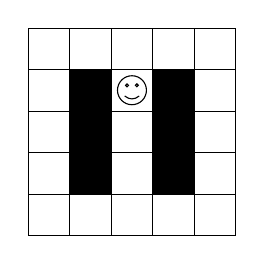
\begin{tikzpicture}[x=0.75pt,y=0.75pt,yscale=-1,xscale=1]
%uncomment if require: \path (0,235); %set diagram left start at 0, and has height of 235

%Shape: Grid [id:dp7926667189539607]
\draw  [draw opacity=0] (205.67,49.33) -- (305.67,49.33) -- (305.67,149.33) -- (205.67,149.33) -- cycle ; \draw   (225.67,49.33) -- (225.67,149.33)(245.67,49.33) -- (245.67,149.33)(265.67,49.33) -- (265.67,149.33)(285.67,49.33) -- (285.67,149.33) ; \draw   (205.67,69.33) -- (305.67,69.33)(205.67,89.33) -- (305.67,89.33)(205.67,109.33) -- (305.67,109.33)(205.67,129.33) -- (305.67,129.33) ; \draw   (205.67,49.33) -- (305.67,49.33) -- (305.67,149.33) -- (205.67,149.33) -- cycle ;
%Shape: Rectangle [id:dp8391924204825284]
\draw  [fill={rgb, 255:red, 0; green, 0; blue, 0 }  ,fill opacity=1 ] (225.67,109.33) -- (245.67,109.33) -- (245.67,129.33) -- (225.67,129.33) -- cycle ;
%Shape: Rectangle [id:dp2074798919794021]
\draw  [fill={rgb, 255:red, 0; green, 0; blue, 0 }  ,fill opacity=1 ] (225.67,89.33) -- (245.67,89.33) -- (245.67,109.33) -- (225.67,109.33) -- cycle ;
%Shape: Rectangle [id:dp6068250248976063]
\draw  [fill={rgb, 255:red, 0; green, 0; blue, 0 }  ,fill opacity=1 ] (225.67,69.33) -- (245.67,69.33) -- (245.67,89.33) -- (225.67,89.33) -- cycle ;
%Shape: Rectangle [id:dp35143600318814394]
\draw  [fill={rgb, 255:red, 0; green, 0; blue, 0 }  ,fill opacity=1 ] (265.67,109.33) -- (285.67,109.33) -- (285.67,129.33) -- (265.67,129.33) -- cycle ;
%Shape: Rectangle [id:dp02419663980472353]
\draw  [fill={rgb, 255:red, 0; green, 0; blue, 0 }  ,fill opacity=1 ] (265.67,89.33) -- (285.67,89.33) -- (285.67,109.33) -- (265.67,109.33) -- cycle ;
%Shape: Rectangle [id:dp8069614076610544]
\draw  [fill={rgb, 255:red, 0; green, 0; blue, 0 }  ,fill opacity=1 ] (265.67,69.33) -- (285.67,69.33) -- (285.67,89.33) -- (265.67,89.33) -- cycle ;
%Shape: Smiley Face [id:dp11055548877169996]
\draw   (248.67,79.2) .. controls (248.67,75.35) and (251.79,72.22) .. (255.64,72.22) .. controls (259.5,72.22) and (262.62,75.35) .. (262.62,79.2) .. controls (262.62,83.05) and (259.5,86.18) .. (255.64,86.18) .. controls (251.79,86.18) and (248.67,83.05) .. (248.67,79.2) -- cycle ; \draw   (252.57,76.83) .. controls (252.57,76.44) and (252.89,76.13) .. (253.27,76.13) .. controls (253.66,76.13) and (253.97,76.44) .. (253.97,76.83) .. controls (253.97,77.21) and (253.66,77.53) .. (253.27,77.53) .. controls (252.89,77.53) and (252.57,77.21) .. (252.57,76.83) -- cycle ; \draw   (257.32,76.83) .. controls (257.32,76.44) and (257.63,76.13) .. (258.02,76.13) .. controls (258.4,76.13) and (258.71,76.44) .. (258.71,76.83) .. controls (258.71,77.21) and (258.4,77.53) .. (258.02,77.53) .. controls (257.63,77.53) and (257.32,77.21) .. (257.32,76.83) -- cycle ; \draw   (252.16,81.99) .. controls (254.48,83.85) and (256.81,83.85) .. (259.13,81.99) ;
\end{tikzpicture}


En este caso, el robot no sabe si debería seguir la pared a su este o a su oeste.
\end{center}

Por ejemplo, tengamos el siguiente mundo:

\begin{center}
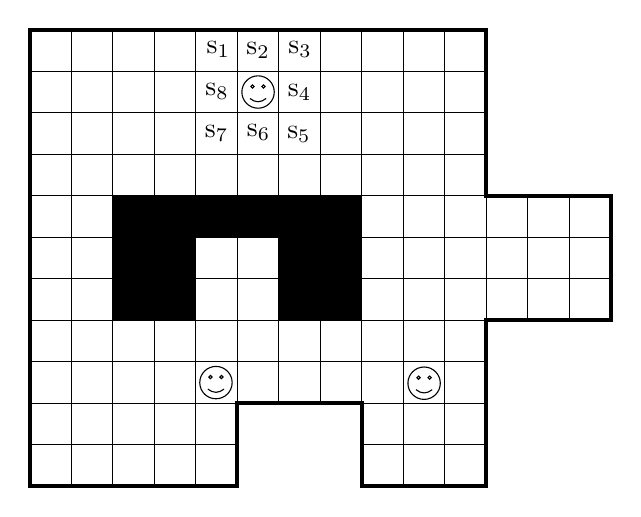
\begin{tikzpicture}[x=0.75pt,y=0.75pt,yscale=-1,xscale=1]
%uncomment if require: \path (0,235); %set diagram left start at 0, and has height of 235

%Shape: Grid [id:dp2475578602604389]
\draw  [draw opacity=0] (182.29,3.14) -- (402.29,3.14) -- (402.29,183.14) -- (182.29,183.14) -- cycle ; \draw   (202.29,3.14) -- (202.29,183.14)(222.29,3.14) -- (222.29,183.14)(242.29,3.14) -- (242.29,183.14)(262.29,3.14) -- (262.29,183.14)(282.29,3.14) -- (282.29,183.14)(302.29,3.14) -- (302.29,183.14)(322.29,3.14) -- (322.29,183.14)(342.29,3.14) -- (342.29,183.14)(362.29,3.14) -- (362.29,183.14)(382.29,3.14) -- (382.29,183.14) ; \draw   (182.29,23.14) -- (402.29,23.14)(182.29,43.14) -- (402.29,43.14)(182.29,63.14) -- (402.29,63.14)(182.29,83.14) -- (402.29,83.14)(182.29,103.14) -- (402.29,103.14)(182.29,123.14) -- (402.29,123.14)(182.29,143.14) -- (402.29,143.14)(182.29,163.14) -- (402.29,163.14) ; \draw   (182.29,3.14) -- (402.29,3.14) -- (402.29,183.14) -- (182.29,183.14) -- cycle ;
%Shape: Grid [id:dp4853807189700099]
\draw  [draw opacity=0] (182.29,183.14) -- (282.29,183.14) -- (282.29,223.14) -- (182.29,223.14) -- cycle ; \draw   (202.29,183.14) -- (202.29,223.14)(222.29,183.14) -- (222.29,223.14)(242.29,183.14) -- (242.29,223.14)(262.29,183.14) -- (262.29,223.14) ; \draw   (182.29,203.14) -- (282.29,203.14) ; \draw   (182.29,183.14) -- (282.29,183.14) -- (282.29,223.14) -- (182.29,223.14) -- cycle ;
%Shape: Grid [id:dp8187458749641342]
\draw  [draw opacity=0] (342.29,183.14) -- (402.29,183.14) -- (402.29,223.14) -- (342.29,223.14) -- cycle ; \draw   (362.29,183.14) -- (362.29,223.14)(382.29,183.14) -- (382.29,223.14) ; \draw   (342.29,203.14) -- (402.29,203.14) ; \draw   (342.29,183.14) -- (402.29,183.14) -- (402.29,223.14) -- (342.29,223.14) -- cycle ;
%Shape: Grid [id:dp4434147164533886]
\draw  [draw opacity=0] (402.29,83.14) -- (462.29,83.14) -- (462.29,143.14) -- (402.29,143.14) -- cycle ; \draw   (422.29,83.14) -- (422.29,143.14)(442.29,83.14) -- (442.29,143.14) ; \draw   (402.29,103.14) -- (462.29,103.14)(402.29,123.14) -- (462.29,123.14) ; \draw   (402.29,83.14) -- (462.29,83.14) -- (462.29,143.14) -- (402.29,143.14) -- cycle ;
%Shape: Rectangle [id:dp506112757226649]
\draw  [fill={rgb, 255:red, 0; green, 0; blue, 0 }  ,fill opacity=1 ] (222.29,123.14) -- (242.29,123.14) -- (242.29,143.14) -- (222.29,143.14) -- cycle ;
%Shape: Rectangle [id:dp5538496652738457]
\draw  [fill={rgb, 255:red, 0; green, 0; blue, 0 }  ,fill opacity=1 ] (242.29,83.14) -- (262.29,83.14) -- (262.29,103.14) -- (242.29,103.14) -- cycle ;
%Shape: Rectangle [id:dp7949108809431658]
\draw  [fill={rgb, 255:red, 0; green, 0; blue, 0 }  ,fill opacity=1 ] (222.29,83.14) -- (242.29,83.14) -- (242.29,103.14) -- (222.29,103.14) -- cycle ;
%Shape: Rectangle [id:dp008693408469896413]
\draw  [fill={rgb, 255:red, 0; green, 0; blue, 0 }  ,fill opacity=1 ] (222.29,103.14) -- (242.29,103.14) -- (242.29,123.14) -- (222.29,123.14) -- cycle ;
%Shape: Rectangle [id:dp07198214391706903]
\draw  [fill={rgb, 255:red, 0; green, 0; blue, 0 }  ,fill opacity=1 ] (242.29,103.14) -- (262.29,103.14) -- (262.29,123.14) -- (242.29,123.14) -- cycle ;
%Shape: Rectangle [id:dp48901729947584394]
\draw  [fill={rgb, 255:red, 0; green, 0; blue, 0 }  ,fill opacity=1 ] (302.29,103.14) -- (322.29,103.14) -- (322.29,123.14) -- (302.29,123.14) -- cycle ;
%Shape: Rectangle [id:dp8560568214721641]
\draw  [fill={rgb, 255:red, 0; green, 0; blue, 0 }  ,fill opacity=1 ] (322.29,103.14) -- (342.29,103.14) -- (342.29,123.14) -- (322.29,123.14) -- cycle ;
%Shape: Rectangle [id:dp5167670671739085]
\draw  [fill={rgb, 255:red, 0; green, 0; blue, 0 }  ,fill opacity=1 ] (242.29,123.14) -- (262.29,123.14) -- (262.29,143.14) -- (242.29,143.14) -- cycle ;
%Shape: Rectangle [id:dp3099735057939933]
\draw  [fill={rgb, 255:red, 0; green, 0; blue, 0 }  ,fill opacity=1 ] (262.29,83.14) -- (282.29,83.14) -- (282.29,103.14) -- (262.29,103.14) -- cycle ;
%Shape: Rectangle [id:dp665570471332241]
\draw  [fill={rgb, 255:red, 0; green, 0; blue, 0 }  ,fill opacity=1 ] (282.29,83.14) -- (302.29,83.14) -- (302.29,103.14) -- (282.29,103.14) -- cycle ;
%Shape: Rectangle [id:dp5824069771147012]
\draw  [fill={rgb, 255:red, 0; green, 0; blue, 0 }  ,fill opacity=1 ] (302.29,83.14) -- (322.29,83.14) -- (322.29,103.14) -- (302.29,103.14) -- cycle ;
%Shape: Rectangle [id:dp9419631737421521]
\draw  [fill={rgb, 255:red, 0; green, 0; blue, 0 }  ,fill opacity=1 ] (322.29,123.14) -- (342.29,123.14) -- (342.29,143.14) -- (322.29,143.14) -- cycle ;
%Shape: Rectangle [id:dp9495474914021746]
\draw  [fill={rgb, 255:red, 0; green, 0; blue, 0 }  ,fill opacity=1 ] (302.29,123.14) -- (322.29,123.14) -- (322.29,143.14) -- (302.29,143.14) -- cycle ;
%Shape: Rectangle [id:dp9266769812137341]
\draw  [fill={rgb, 255:red, 0; green, 0; blue, 0 }  ,fill opacity=1 ] (322.29,83.14) -- (342.29,83.14) -- (342.29,103.14) -- (322.29,103.14) -- cycle ;
%Straight Lines [id:da48539602747701405]
\draw [line width=1.5]    (182.29,3.14) -- (182.29,223.14) -- (282.29,223.14) -- (282.29,183.14) -- (342.29,183.14) -- (342.29,223.14) -- (402.29,223.14) -- (402.29,143.14) -- (462.29,143.14) -- (462.29,83.14) -- (402.29,83.14) -- (402.29,3.14) -- cycle ;
%Shape: Smiley Face [id:dp58077148066748]
\draw   (284.49,33.14) .. controls (284.49,28.84) and (287.98,25.34) .. (292.29,25.34) .. controls (296.59,25.34) and (300.09,28.84) .. (300.09,33.14) .. controls (300.09,37.45) and (296.59,40.94) .. (292.29,40.94) .. controls (287.98,40.94) and (284.49,37.45) .. (284.49,33.14) -- cycle ; \draw   (288.85,30.49) .. controls (288.85,30.06) and (289.2,29.71) .. (289.63,29.71) .. controls (290.06,29.71) and (290.41,30.06) .. (290.41,30.49) .. controls (290.41,30.92) and (290.06,31.27) .. (289.63,31.27) .. controls (289.2,31.27) and (288.85,30.92) .. (288.85,30.49) -- cycle ; \draw   (294.16,30.49) .. controls (294.16,30.06) and (294.51,29.71) .. (294.94,29.71) .. controls (295.37,29.71) and (295.72,30.06) .. (295.72,30.49) .. controls (295.72,30.92) and (295.37,31.27) .. (294.94,31.27) .. controls (294.51,31.27) and (294.16,30.92) .. (294.16,30.49) -- cycle ; \draw   (288.39,36.26) .. controls (290.99,38.34) and (293.59,38.34) .. (296.19,36.26) ;
%Shape: Smiley Face [id:dp2710696886885271]
\draw   (264.2,173.14) .. controls (264.2,168.84) and (267.69,165.34) .. (272,165.34) .. controls (276.31,165.34) and (279.8,168.84) .. (279.8,173.14) .. controls (279.8,177.45) and (276.31,180.94) .. (272,180.94) .. controls (267.69,180.94) and (264.2,177.45) .. (264.2,173.14) -- cycle ; \draw   (268.57,170.49) .. controls (268.57,170.06) and (268.92,169.71) .. (269.35,169.71) .. controls (269.78,169.71) and (270.13,170.06) .. (270.13,170.49) .. controls (270.13,170.92) and (269.78,171.27) .. (269.35,171.27) .. controls (268.92,171.27) and (268.57,170.92) .. (268.57,170.49) -- cycle ; \draw   (273.87,170.49) .. controls (273.87,170.06) and (274.22,169.71) .. (274.65,169.71) .. controls (275.08,169.71) and (275.43,170.06) .. (275.43,170.49) .. controls (275.43,170.92) and (275.08,171.27) .. (274.65,171.27) .. controls (274.22,171.27) and (273.87,170.92) .. (273.87,170.49) -- cycle ; \draw   (268.1,176.26) .. controls (270.7,178.34) and (273.3,178.34) .. (275.9,176.26) ;
%Shape: Smiley Face [id:dp7945056589510564]
\draw   (364.49,173.43) .. controls (364.49,169.12) and (367.98,165.63) .. (372.29,165.63) .. controls (376.59,165.63) and (380.09,169.12) .. (380.09,173.43) .. controls (380.09,177.74) and (376.59,181.23) .. (372.29,181.23) .. controls (367.98,181.23) and (364.49,177.74) .. (364.49,173.43) -- cycle ; \draw   (368.85,170.78) .. controls (368.85,170.35) and (369.2,170) .. (369.63,170) .. controls (370.06,170) and (370.41,170.35) .. (370.41,170.78) .. controls (370.41,171.21) and (370.06,171.56) .. (369.63,171.56) .. controls (369.2,171.56) and (368.85,171.21) .. (368.85,170.78) -- cycle ; \draw   (374.16,170.78) .. controls (374.16,170.35) and (374.51,170) .. (374.94,170) .. controls (375.37,170) and (375.72,170.35) .. (375.72,170.78) .. controls (375.72,171.21) and (375.37,171.56) .. (374.94,171.56) .. controls (374.51,171.56) and (374.16,171.21) .. (374.16,170.78) -- cycle ; \draw   (368.39,176.55) .. controls (370.99,178.63) and (373.59,178.63) .. (376.19,176.55) ;

% Text Node
\draw (273.14,12.57) node   [align=left] {s\textsubscript{1}};
% Text Node
\draw (292.29,13.14) node   [align=left] {s\textsubscript{2}};
% Text Node
\draw (312.57,12.86) node   [align=left] {s\textsubscript{3}};
% Text Node
\draw (272.57,32.86) node   [align=left] {s\textsubscript{8}};
% Text Node
\draw (272.29,53.14) node   [align=left] {s\textsubscript{7}};
% Text Node
\draw (292.57,52.86) node   [align=left] {s\textsubscript{6}};
% Text Node
\draw (312.29,33.43) node   [align=left] {s\textsubscript{4}};
% Text Node
\draw (312,53.43) node   [align=left] {s\textsubscript{5}};
\end{tikzpicture}


Los bordes gruesos representan los límites del mundo y el área opaca, un objeto sólido.
\end{center}

Un robot escaneará sus ocho casillas colindantes buscando cuáles están libres para ocupar, como hace el robot superior.
Un robot que comience en la posición del robot inferior izquierdo avanzará en sentido contrario a las ajugas del reloj a lo largo del limite del mundo.
Un robot que comience en la posición del robot inferior derecho avanzará a la derecha para seguir avanzando en sentido de las ajugas del rejor a lo largo del límite del mundo.

Dado este mundo con dos robots $A$ y $B$, podemos representarlo fácilmente en una matriz:

\begin{lstlisting}[language=C]
char mundo[16][13] =
	{1,1,1,1,1,1,1,1,1,1,1,1,1,1,1,1}
	{1,0,0,0,0,0,0,0,0,0,0,0,1,1,1,1}
	{1,0,0,0,0,0,0,0,0,0,0,0,1,1,1,1}
	{1,0,0,0,0,0,0,0,0,0,0,0,1,1,1,1}
	{1,0,0,0,0,0,0,0,0,0,0,0,1,1,1,1}
	{1,0,0,1,1,1,1,1,1,0,0,0,0,0,0,1}
	{1,0,0,1,1,0,0,1,1,0,0,0,0,0,0,1}
	{1,0,0,1,1,0,0,1,1,0,0,0,0,0,0,1}
	{1,0,0,0,0,0,0,0,0,0,0,0,1,1,1,1}
	{1,0,0,0,0,A,0,0,0,0,B,0,1,1,1,1}
	{1,0,0,0,0,0,1,1,1,0,0,0,1,1,1,1}
	{1,0,0,0,0,0,1,1,1,0,0,0,1,1,1,1}
	{1,1,1,1,1,1,1,1,1,1,1,1,1,1,1,1};

int sensores[8];
\end{lstlisting}

\pagebreak

Los \code{sensores} podemos representarlos como un vector de 8 compoenentes.
Este vector tendría el siguiente estado en la posición del robot $A$:

\[\big(0,0,0,0,1,0,0,0\big)\]

Definimos también cuatro movimientos posibles:

\begin{itemize}
	\item\textbf{Norte:} Mover el robot una casilla hacia arriba.
	\item\textbf{Sur:} Mover el robot una casill hacia abajo.
	\item\textbf{Este:} Mover el robot una casilla hacia la derecha.
	\item\textbf{Oste:} Mover el robot una casilla hacia la izquierda.
\end{itemize}

Tras estas definiciones, queda como trabajo del diseñador del robot desarrollar una función que tome las entradas sensoriales del mundo y seleccione la opción apropiada en cada caso para llevar a cabo exitosamente la tarea del robot.

\subsection{Un proceso en dos fases}

Cada acción que realiza el agente reactivo está dividida en dos fases que unidas por una estructura de datos común.

\subsubsection{Primera fase: Proceso perceptivo}

En esta fase el agente recibe estímulos a través de sus entradas sensoriales y, mediante un proceso de digitalización, los almacena en una estructura de datos.
En el ejemplo anterior, los espacios adyacentes al agente recibidos mediante las entradas sensoriales se almacenan digitalmente en un vector de ocho componentes.

\subsubsection{Segunda fase: Función de acción}

Tras recibir y almacenar la información de su entorno, el agente analiza dicha informacion y realiza acciones acordes con ella.
En el caso del vector en el que un \code{0} simboliza un espacio libre y un \code{1} simboliza un espacio ocupado, el agente no intentará moverse hacia los espacios ocupados, ya que fracasaría.

De la misma forma, podemos definir a qué espacio debe moverse el robot en función de las casillas libres.
Simplificando el vector a cuatro componentes \code{norte}, \code{este}, \code{sur} y \code{oeste}, podríamos definir los movimientos del agente en función de sus valores\footnote{Estas definiciones pueden o no seguir una lógica. En el caso de esta tabla, se han definido de forma que todas las direcciones tengan más o menos la misma presencia, pero el resultado podría haber sido cualquier otro teniendo en cuenta las restricciones espaciales.}:

\begin{center}
\begin{tabular}{c c c c l c c c c l}
$\boldsymbol{N}$ & $\boldsymbol{E}$ & $\boldsymbol{S}$ & $\boldsymbol{W}$ & \textbf{Movimiento} & $\boldsymbol{N}$ & $\boldsymbol{E}$ & $\boldsymbol{S}$ & $\boldsymbol{W}$ & \textbf{Movimiento} \\
\toprule
$0$ & $0$ & $0$ & $0$ & Norte & $1$ & $0$ & $0$ & $0$ & Este  \\
$0$ & $0$ & $0$ & $1$ & Norte & $1$ & $0$ & $0$ & $1$ & Este  \\
$0$ & $0$ & $1$ & $0$ & Oeste & $1$ & $0$ & $1$ & $0$ & Este  \\
$0$ & $0$ & $1$ & $1$ & Norte & $1$ & $0$ & $1$ & $1$ & Este  \\
$0$ & $1$ & $0$ & $0$ & Sur   & $1$ & $1$ & $0$ & $0$ & Sur   \\
$0$ & $1$ & $0$ & $1$ & Sur   & $1$ & $1$ & $0$ & $1$ & Sur   \\
$0$ & $1$ & $1$ & $0$ & Oeste & $1$ & $1$ & $1$ & $0$ & Oeste \\
$0$ & $1$ & $1$ & $1$ & Norte & $1$ & $1$ & $1$ & $1$ & ---   \\
\end{tabular}
\end{center}

\subsection{Arquitecturas de agentes reactivos}

\subsubsection{Sistemas de producción}

A la hora de diseñar un agente reactivo lo hacemos mediante un sistema de aplicaciones que, a partir de una serie de funciones booleanas $c_k$, se active una función de acción $a_k$.

\[c_1\rightarrow a_1,\ c_2\rightarrow a_2,\ \cdots,\ c_{i-1}\rightarrow a_{i-1},\ c_i\rightarrow a_i\]

En el ejemplo anterior, llamemos $x_1$ a la presencia de un obstáculo al norte del agente y $\overline{x_1}$ a la ausencia del mismo.
Hagamos lo mismo para el este ($x_2$), sur ($x_3$) y oeste ($x_4$).
De esta forma, podríamos expresar algunos de los movimientos mediante funciones booleanas:

\[0\rightarrow Norte,\ \overline{x_0}\overline{x_1}\overline{x_2}x_3\rightarrow Norte,\ x_0x_1x_2\overline{x_3}\rightarrow Oeste,\ 1\rightarrow \text{---}\]

\subsubsection{Redes neuronales}

Una forma más compleja de definir estas arquitecturas es mediante redes neuronales.
Las redes neuronales están compuestas por conjuntos de puertas umbrales, llamadas neuronas, que evalúan los estímulos dando a cada uno de ellos un peso.
Cuanto más alto es el peso de un estímulo, más determinante es su valor a la hora de calcular la salida de la puerta umbral

\begin{figure}[h]
\begin{center}
% Listing 2: Tex for neural network pipeline
\begin{tikzpicture}[
    % define styles
    init/.style={%
         draw,
         circle,
         inner sep=2pt,
         font=\Huge,
         join = by -latex
    },
    squa/.style={%
        font=\Large,
        join = by -latex
    }
]% Top chain x1 to w1
\begin{scope}[start chain=1]
    \node[on chain=1] at (0,1.5cm)  (x1) {$x_1$};
    \node[on chain=1,join=by o-latex] (w1) {$w_1$};
\end{scope}% Middle chain x2 to output

\begin{scope}[start chain=2]
    \node[on chain=2] (x2) {$x_2$};
    \node[on chain=2,join=by o-latex] {$w_2$};
    \node[on chain=2,init] (sigma) {$\displaystyle\Sigma$};
    \node[on chain=2,squa,label=above:Salida,join=by -latex] {$f$};
\end{scope}% Bottom chain x3 to w3

\begin{scope}[start chain=3]
    \node[on chain=3] at (0,-1.5cm)
    (x3) {$x_3$};
    \node[on chain=3,label=below:Pesos,join=by o-latex]
    (w3) {$w_3$};
\end{scope}% Bias

	\node[label=above:\parbox{2cm}{\centering Suma ponderada \\ $\sum_{i=1}^{k}x_kw_k$}] at (sigma|-w1) (b) {};% Arrows joining w1, w3 and b to sigma
\draw[-latex] (w1) -- (sigma);
\draw[-latex] (w3) -- (sigma);
\draw[o-latex] (b) -- (sigma);% left hand side brace
\draw[decorate,decoration={brace,mirror}] (x1.north west) -- node[left=10pt] {Entrada} (x3.south west);
\end{tikzpicture}
	\caption{Neurona que, mediante estímulos $x_i$ con peso $w_i$, genera una salida $f$.}
\end{center}
\end{figure}

A través de un sistema complejo de neuronas, la red evalúa todos los estímulos y genera una salida.

\begin{figure}[h]
\begin{center}

\end{center}
\caption{Diseño de una red neuronal (Por implementar)}
\end{figure}

\subsubsection{Arquitecturas de subsunción}

La arquitectura de subsunción agrupa módulos de comportamiento de forma que las acciones estén organizadas en una jerarquía de ejecución.
Si un módulo superior del esquema se cumple, se ejecuta en lugar de los módulos inferiores.

\subsection{Agentes reactivos con memoria}

Hasta ahora hemos estado trabajado con agentes que toman decisiones basándose únicamente en el estado de su entorno en el presente más inmediato.
Estos agentes tienen como limitación que no pueden tomar decisiones en función de la decisión tomada anteriormente.
Por ejemplo, un agente que al salir de un pasillo estrecho girará siempre a la derecha, deberá recordar que antes se encontraba en un pasillo estrecho (hace dos instantes percibió dos espacios ocupados al norte y sur o al este y oeste) y que en el instante anterior salió del pasillo, encontrándose en el espacio inmediatamente posterior al mismo.

Para este tipo de problemas existen los sistemas con memoria, en cuyo proceso perceptivo tienen en cuenta tanto la entrada sensorial como la información de los instantes anteriores almacenada en memoria.

\subsubsection{Representaciones icónicas}

Podemos implementar la memoria con estructuras de datos diferentes a la percibida por la entrada sensorial.
Por ejemplo, podemos hacer que éste almacene una matriz que contenga el estado de cada espacio en el momento en el que se percibieron.

\section{Campo de potencial artificial}

Iyo no sé
